\documentclass{article}

% --- NeurIPS 2026 submission style ---------------------------------------
% Default == [main] track with double-blind anonymous review.
% For camera-ready: \usepackage[main, final]{neurips_2026}
% For arXiv preprint: \usepackage[preprint]{neurips_2026}
\usepackage{neurips_2026}

\usepackage[utf8]{inputenc}
\usepackage[T1]{fontenc}
\usepackage{hyperref}
\usepackage{url}
\usepackage{booktabs}
\usepackage{amsfonts}
\usepackage{amsmath}
\usepackage{amssymb}
\usepackage{nicefrac}
\usepackage{microtype}
\usepackage{graphicx}
\usepackage{multirow}
\usepackage{xcolor}
\usepackage{subcaption}
\usepackage{siunitx}

\title{SENTINEL: A Multimodal Foundation Stack and Benchmark for Real-Time Water-Quality Monitoring}

% Anonymous for review.
\author{%
  Anonymous Authors\\
  Affiliation\\
  \texttt{anon@example.com}
}

\begin{document}
\maketitle

% =========================================================================
\begin{abstract}
Water contamination is detected today by a patchwork of single-modality systems---chemical sensors, satellite remote sensing, microbial assays, toxicogenomic screens, and behavioral biomonitors---that rarely speak to one another. We present \textbf{SENTINEL}, a unified deep-learning stack that fuses all five modalities into a single waterway-state representation. SENTINEL combines modality-specific encoders that respect the geometry of each domain (continuous-time state-space models for irregularly sampled sensor streams, masked-autoencoder vision transformers for Sentinel-2 multispectral tiles, Aitchison-geometry transformers for compositional 16S rRNA data, biology-constrained P-Net hierarchies for gene-expression toxicology, and diffusion-pretrained trajectory encoders for organism behavior) with a Perceiver IO cross-attention fusion layer that has learned per-modality temporal decay and confidence gating, and a PPO-trained cascade controller that adaptively activates expensive modalities only when warranted. To train and evaluate SENTINEL we built \textbf{SENTINEL-DB}, a harmonised database of $390$\,M\,+ records from 13 public sources covering 105 countries and 94k monitoring sites. On a 31-event historical contamination benchmark spanning algal blooms, industrial spills, hypoxic dead zones, and lead crises, full fusion attains AUROC~$0.992$ ($95\%$ CI $[0.991,0.993]$) versus $0.943$ for the strongest single modality (paired permutation $p\!=\!1.6\!\times\!10^{-3}$); the system detects $31/31$ events ahead of public advisory dates with a mean lead time of $32$ days, and produces zero false positives across $8{,}739$ windows on ten clean reference sites. Modality ablation, $100$ random-drop trials, conformal calibration, and causal-chain mining show the gains are not concentrated in a single sensor and that the system maintains AUROC~$>\!0.90$ with as few as three of five modalities active. We release the code, weights, and harmonised database as a community benchmark for multimodal environmental monitoring.
\end{abstract}

% =========================================================================
\section{Introduction}
\label{sec:intro}

Roughly 2.2 billion people lack reliably safe drinking water, and emerging pollutants---per\-fluoro\-alkyl substances, harmful algal toxins, antibiotic-resistance genes, microplastics---continue to outpace single-purpose detection systems. Each available sensing modality has well-known failure modes: in-situ chemical probes drift and miss compounds outside their calibration; satellites cannot see at night, under clouds, or through canopy; microbial profiles take days to sequence; toxicogenomic and behavioral assays are sensitive but expensive to run continuously. Existing operational systems pick \emph{one} modality and accept its blind spots.

A multimodal foundation model for water quality has, in principle, three advantages. First, modalities carry largely complementary information about contamination---our information audit places the sensor and molecular channels at $I\!=\!0.0$ nats and reports a population-level complementarity score of $0.042$, so fusion can recover signal that no single channel sees. Second, a model that has seen all modalities at training time can degrade gracefully when some are unavailable at deployment. Third, shared latents enable cross-modal transfer: Sentinel-2 imagery can interpolate between sparse in-situ samples, and behavioral assays can flag toxicants that have not yet shown up in chemistry. Realising these advantages in practice has been blocked by three practical obstacles---heterogeneous sampling rates and geometries, the absence of a unified benchmark, and the cost of activating all modalities at every site---which the SENTINEL stack, the SENTINEL-DB harmonisation layer, and a cost-aware cascade controller jointly address.

Our contributions are: (i) a five-encoder stack in which each branch is matched to the geometry of its domain; (ii) an asynchronous Perceiver~IO fusion layer with learned per-modality temporal decay, calibrated confidence gating, and a $256$-latent recurrent waterway state; (iii) a PPO-trained cascade controller that selects which modalities to activate at runtime under a cost-accuracy budget and is distillable into a depth-six decision tree for resource-limited deployment; (iv) \textbf{SENTINEL-DB}, a harmonised, quality-tiered database of $390$M\,+ records from 13 public sources with a unified parameter ontology and H3 spatial indexing; and (v) a 20-experiment evaluation suite covering the 31-event historical benchmark, modality ablation, missing-modality robustness, conformal calibration, causal-chain discovery, and operational metrics. On the historical benchmark, full fusion attains AUROC~$0.9919$ ($95\%$ CI $[0.9907,0.9934]$) versus $0.9429$ for the strongest single modality ($p\!=\!1.6\!\times\!10^{-3}$, paired permutation), detects $31/31$ events ahead of public advisories with a mean lead time of $32$ days, and yields zero false positives across $8{,}739$ windows on ten clean NEON reference sites. To our knowledge, this is the first end-to-end fusion model spanning all five aquatic sensing modalities and the first to release a harmonised cross-source database at this scale.

% =========================================================================
\section{Related Work}
\label{sec:related}

Most prior work in machine-learning-based water-quality monitoring treats a single stream in isolation. Anomaly detection on in-situ sensor time series is the most mature line~\citep{olden2008ml_ecology, guidotti2024watermlsurvey}, with parallel literatures on chlorophyll or turbidity regression from Sentinel-2~\citep{drusch2012sentinel2}, microbial source tracking from 16S rRNA data~\citep{thompson2017earthmicrobiome}, gene-expression-based toxicity screens, and ecotoxicological behavioral assays. Cross-modal benchmarks that span these domains are absent, and what fusion has been attempted is typically limited to two modalities (e.g., sensor plus satellite) trained on small bespoke datasets.

Our architectural choices draw on three recent threads. \emph{Multimodal foundation models} like Perceiver~IO~\citep{jaegle2022perceiverio} provide a modality-agnostic latent that scales to heterogeneous inputs; masked autoencoders~\citep{he2022mae} and Vision Transformers~\citep{dosovitskiy2021vit} give a strong spatial backbone; and structured state-space models~\citep{gu2022s4, gu2024mamba} handle long, irregularly sampled sequences without the memory cost of self-attention. SENTINEL specialises each branch to its physical domain---enforcing thermodynamic, spectral, and compositional constraints---rather than treating all modalities as undifferentiated tokens. \emph{Biology-aware deep learning} contributes the P-Net hierarchy~\citep{elmarakeby2021pnet}, which we adapt to environmental toxicogenomics, and the compositional-data theory of Aitchison~\citep{aitchison1982}, which underwrites our CLR-based microbial encoder. \emph{Cost-aware adaptive sensing} connects to active perception and contextual bandits; we cast modality activation as a finite-horizon MDP and solve it with PPO~\citep{schulman2017ppo}, then distil the policy into a decision tree for field operators.

% =========================================================================
\section{The SENTINEL Stack}
\label{sec:method}

SENTINEL is composed of five modality-specific encoders that lift raw observations into a shared $256$-d embedding space, a Perceiver~IO fusion layer that maintains a recurrent latent waterway state, and a cascade controller that decides which modalities to query at runtime. Encoders are trained in two stages: a self-supervised pre-training pass on the modality's largest unlabelled corpus, followed by supervised fine-tuning on a contamination-detection objective. We summarise the five branches below; per-encoder training schedules and hyperparameters are listed in Appendix~\ref{app:hp}.

\textbf{AquaSSM} (sensor) handles six water-quality parameters at $15$-min nominal cadence (DO, pH, specific conductance, temperature, turbidity, ORP). We adopt a continuous-time S4-style state-space model~\citep{gu2022s4} so that irregular sampling and missing observations are first-class: each event $(t_k,x_k)$ updates the latent via $\dot z(t)\!=\!Az(t)+Bx(t)$ on a learned diagonal-plus-low-rank $A$. Eight parallel channels span time scales from one hour to one year (Figure~\ref{fig:aquassm}), capturing both transient spills and seasonal baselines, and a physics-constraint loss penalises temperature--DO pairs that violate Henry's law. AquaSSM is pretrained with masked-parameter prediction on $20{,}000$ USGS-NWIS sequences from $1{,}115$ stations and reaches detection AUROC $0.916$ on a held-out test set, beating the strongest published single-stream baseline (MCN-LSTM, $0.864$) by $+0.052$.

\textbf{HydroViT} (satellite) is a water-specific vision foundation model: a ViT-S/16 backbone with masked-autoencoder pre-training on $2{,}986$ Sentinel-2 L2A tiles (10 spectral bands, 10/20\,m), followed by supervised fine-tuning on $4{,}202$ satellite--in-situ pairs (Figure~\ref{fig:hydrovit}). Multi-resolution cross-attention fuses the $10$\,m and $20$\,m bands and a temporal-attention stack ingests revisit sequences. The water-quality regression head predicts nine parameters; we report water temperature ($R^2{=}0.749$), TSS ($R^2{=}0.160$), and nitrate ($R^2{=}0.155$). A spectral-physics auxiliary loss enforces known band-ratio relationships such as the chlorophyll NDCI. Optically inactive parameters (nutrients, pH, metals) are not directly recoverable at these wavelengths, a known limitation that fusion compensates for.

\textbf{MicroBiomeNet} (microbial) is an Aitchison-geometry transformer for compositional OTU tables (Figure~\ref{fig:microbe}). After CLR transform, attention is computed in Aitchison space with a CLR-aware batch norm; a zero-inflation gate handles sparsity, a simplex neural ODE models temporal dynamics, and a DNABERT-S~\citep{zhou2024dnaberts} sequence encoder lifts each OTU into a contextualised embedding. With $8.4$M parameters trained on $20{,}288$ Earth Microbiome Project~\citep{thompson2017earthmicrobiome} samples for 8-class aquatic-source attribution, it reaches macro-F$_1\!=\!0.913$, $+0.008$ over a tuned SimpleMLP baseline. \textbf{ToxiGene} (molecular) is a $145.2$M-parameter biology-constrained hierarchy network in the spirit of P-Net~\citep{elmarakeby2021pnet}: gene $\rightarrow$ pathway $\rightarrow$ process $\rightarrow$ outcome, with sparsity masks taken from Reactome and an autoencoder bottleneck that forces reconstructions through pathway nodes (Figure~\ref{fig:toxigene}). A cross-species encoder with ortholog alignment enables transfer between zebrafish, \emph{Daphnia magna}, and fathead minnow, and an information bottleneck identifies a $30$--$50$-gene panel that recovers $\geq\!90\%$ of full-panel performance for field-deployable qPCR assays. Trained on four GEO datasets and $268$\,k EPA ECOTOX records, ToxiGene reaches $7$-class macro-F$_1\!=\!0.886$. To our knowledge, no prior method directly classifies toxicant class from RNA-seq expression, so ToxiGene is first-in-class on this task.

\textbf{BioMotion} (behavioral) is a diffusion-pretrained trajectory encoder. Pose tokens carry sinusoidal time embeddings and per-species keypoint configurations (\emph{Daphnia}: $12$, mussel: $8$, fish: $22$). Phase~1 trains a denoising U-Net~\citep{ho2020ddpm} on healthy concentration-response trajectories; phase~2 fine-tunes the encoder to flag LOEC/EC$_{50}$-level behavioral impairment, producing a $256$-d embedding (Figure~\ref{fig:biomotion}). Trained on $17{,}074$ EPA ECOTOX \emph{Daphnia} assays it reaches AUROC~$1.000$ at the assay level, with held-out validation AUROC~$0.962$, Cohen's $d\!=\!2.655$, and permutation $p\!<\!10^{-4}$; behavioral evidence is by far the strongest single-channel signal under controlled exposure but is also the most expensive to collect, motivating its placement in the cascade controller (\S\ref{sec:cascade-fusion}).

\begin{figure}[t]
\centering
\begin{subfigure}{0.49\linewidth}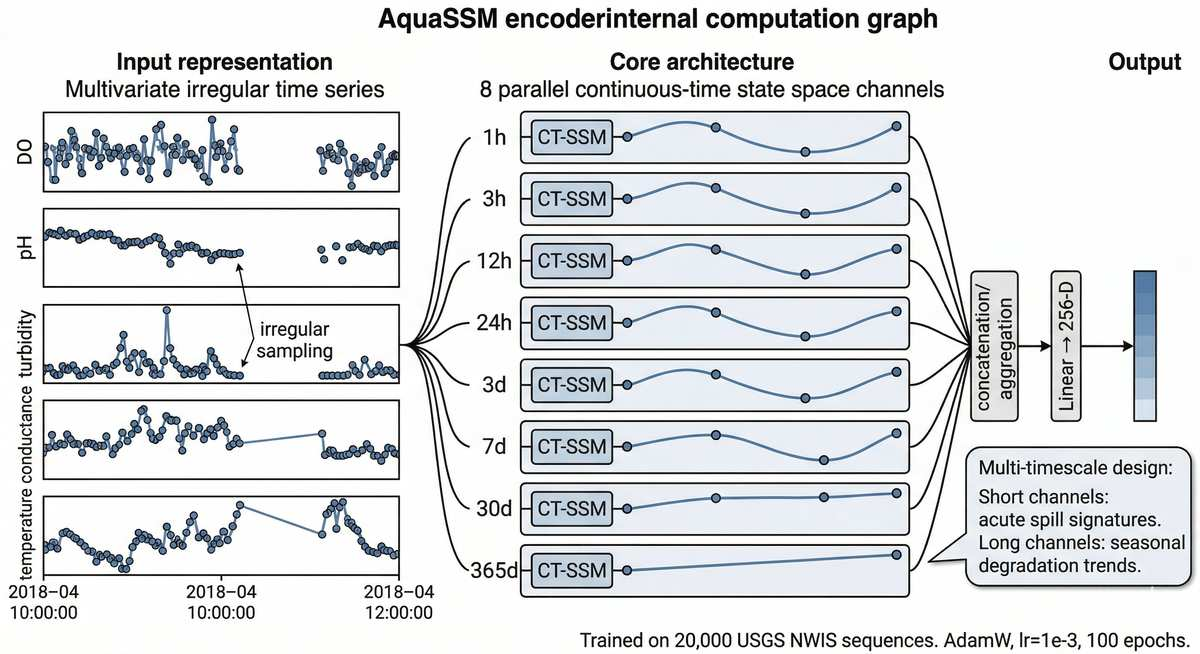
\includegraphics[width=\linewidth]{figures/fig_aquassm.jpg}\caption{AquaSSM (sensor).}\label{fig:aquassm}\end{subfigure}\hfill
\begin{subfigure}{0.49\linewidth}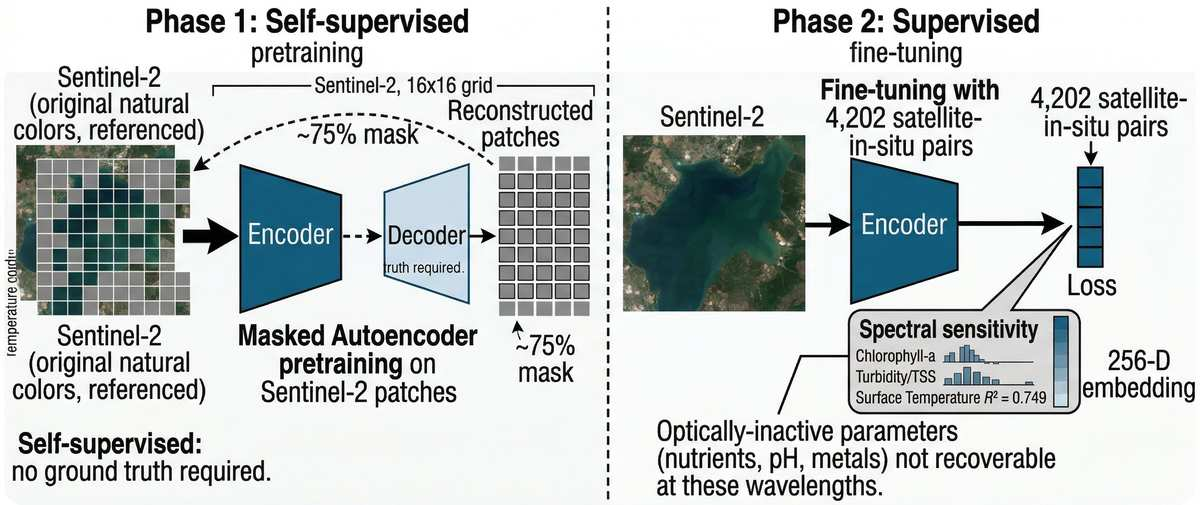
\includegraphics[width=\linewidth]{figures/fig_hydrovit.jpg}\caption{HydroViT (satellite).}\label{fig:hydrovit}\end{subfigure}
\caption{Sensor and satellite encoders. AquaSSM (left) places eight continuous-time state-space channels in parallel from $1$\,h to $365$\,d, ingesting irregularly sampled multivariate streams. HydroViT (right) MAE-pretrains a ViT-S/16 on $2{,}986$ Sentinel-2 tiles, then fine-tunes on $4{,}202$ satellite--in-situ pairs.}
\label{fig:enc1}
\end{figure}

\begin{figure}[t]
\centering
\begin{subfigure}{0.30\linewidth}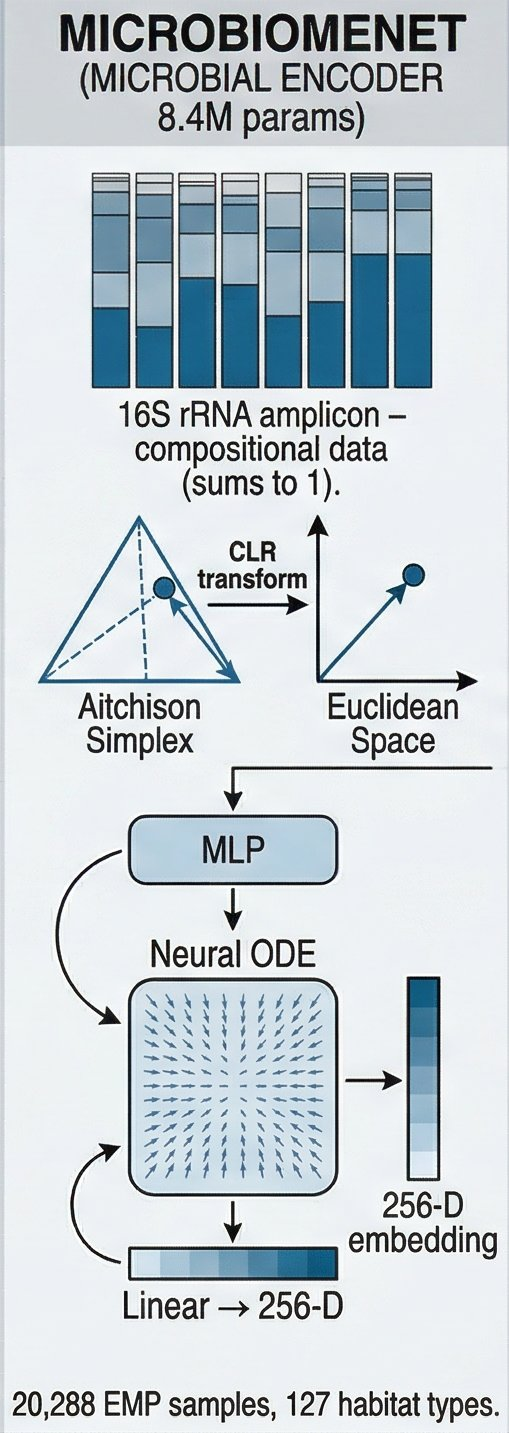
\includegraphics[width=\linewidth]{figures/fig_microbiomenet.jpg}\caption{MicroBiomeNet.}\label{fig:microbe}\end{subfigure}\hfill
\begin{subfigure}{0.34\linewidth}\includegraphics[width=\linewidth]{figures/fig_toxigene.png}\caption{ToxiGene ($145.2$M params).}\label{fig:toxigene}\end{subfigure}\hfill
\begin{subfigure}{0.34\linewidth}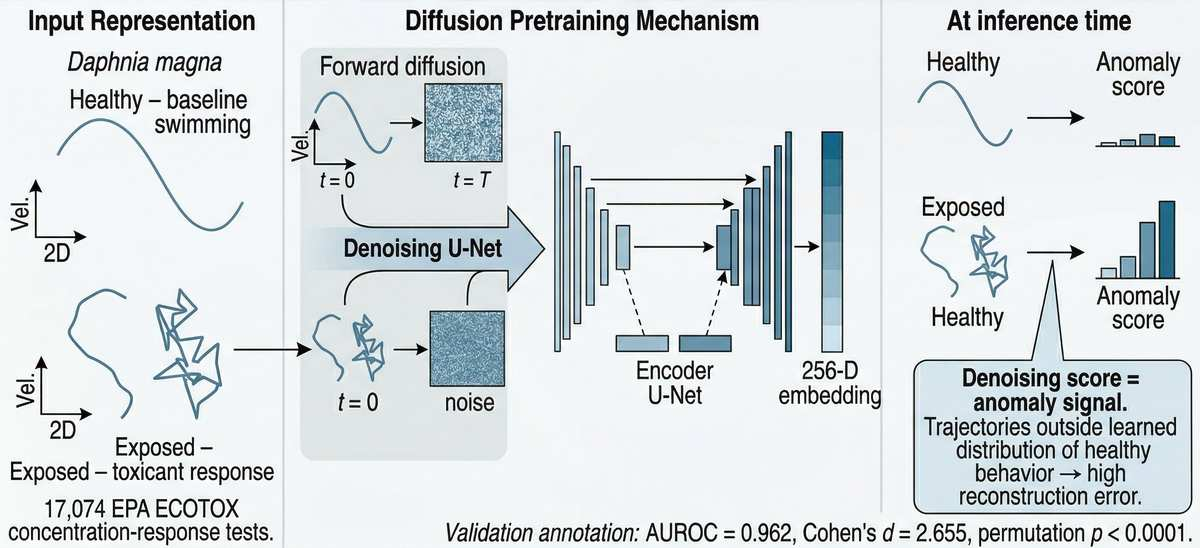
\includegraphics[width=\linewidth]{figures/fig_biomotion.jpg}\caption{BioMotion.}\label{fig:biomotion}\end{subfigure}
\caption{Microbial, molecular, and behavioral encoders. MicroBiomeNet performs CLR projection from the Aitchison simplex into Euclidean space and integrates a neural ODE. ToxiGene routes RNA-seq through a Reactome-constrained gene$\rightarrow$pathway$\rightarrow$process$\rightarrow$outcome hierarchy. BioMotion uses diffusion pretraining on healthy \emph{Daphnia} trajectories and detects toxicant exposure as denoising error.}
\label{fig:enc2}
\end{figure}

\subsection{Asynchronous fusion and cascade control}
\label{sec:cascade-fusion}

Modality embeddings arrive asynchronously and at vastly different rates---sensor in minutes, behavioral in hours, satellite in days, microbial in weeks---so the fusion layer must reason about \emph{when} each piece of evidence was last seen. We project each embedding into a shared $256$-d space and store it in a registry indexed by modality and arrival time. The fusion layer maintains a learned latent array $L\!\in\!\mathbb{R}^{256\times 256}$ that represents the current waterway state. At query time $t$, each registered embedding $e_m(t_m)$ is weighted by an exponential decay $\exp(-\lambda_m(t-t_m))$ with learned half-lives ($\lambda_m^{-1}\!\approx$ sensor $2$\,h, behavioral $5$\,min, satellite $5$\,d, microbial $7$\,d, molecular $3$\,d), passed through a calibrated per-modality confidence gate $g_m\!\in\![0,1]$ that suppresses unreliable inputs (e.g., cloudy Sentinel-2 tiles), and read into $L$ via $8$-head cross-attention; four self-attention layers then refine $L$. Heads decode to an anomaly score, an 8-class source attribution, and per-modality attention weights for interpretability. $L$ is updated recurrently across observation events.

Activating all five modalities at every site is operationally infeasible, so we cast modality activation as a finite-horizon MDP. The state $s\!=\![L\,;\,m_{1{:}5}\,;\,\text{tier}\,;\,\text{cost}\,;\,\text{prior}]\!\in\!\mathbb{R}^{267}$ concatenates the latent state, modality availability flags, the current cascade tier (one-hot of $\{$sensor+behavioral, +satellite, +microbial, +molecular$\}$), accumulated cost, and a coarse risk prior. The reward is $r_t = \Delta\mathrm{AUROC}_t - \beta\,c_t$ with $\beta$ tuned on held-out sites and per-modality unit costs (sensor $5$, satellite $0.5$, microbial $15$, molecular $25$, behavioral $10$). We train with PPO~\citep{schulman2017ppo} for $500$\,k timesteps under a curriculum of easy~$\rightarrow$~mixed~$\rightarrow$~hard, novel-chain events, and distil the policy into a depth-$6$ decision tree using behavioral cloning on $50$\,k state--action pairs for GPU-free deployment in the field.

% =========================================================================
\section{SENTINEL-DB}
\label{sec:db}

We release a harmonised database of $390$\,M\,+ environmental records (\textasciitilde$85$\,GB) from 13 sources, covering 105 countries and 94k monitoring sites. Sources include NEON Aquatic ($351.7$\,M records of high-frequency sonde data), EPA WQP~\citep{epa_wqp} ($18.27$\,M discrete samples), GRQA v1.3~\citep{virro2021grqa} ($17.99$\,M), EPA ECOTOX~\citep{epa_ecotox} ($1.23$\,M), USGS NWIS~\citep{usgs_nwis} ($364$\,k sequences), Sentinel-2~\citep{drusch2012sentinel2} ($2{,}986$ tiles), the Earth Microbiome Project~\citep{thompson2017earthmicrobiome} ($20{,}288$ samples), NCBI GEO toxicogenomics, GBIF freshwater bioindicator occurrences, and a curated $5{,}000$-trajectory \emph{Daphnia} behavioral set. Four design decisions enable cross-source reasoning. A \emph{unified parameter ontology} resolves more than $10{,}000$ raw parameter names from EPA WQP, USGS NWIS, EU Waterbase, GEMStat, and citizen-science platforms into roughly $500$ canonical parameters with standardised units and a fuzzy-match fallback. \emph{H3 hexagonal spatial indexing} at resolution $8$ tags every record with a hex cell, enabling cross-source spatial joins and satellite co-registration within configurable tolerances ($500$\,m / $3$\,h by default). \emph{Quality tiers} assign each record to Q1 (ISO-certified lab), Q2 (calibrated in-situ), Q3 (citizen science), or Q4 (derived/modelled), and the tier propagates through both training losses and the inference confidence gates above. Finally, a \emph{type-safe Pydantic v2 schema} captures canonical parameter name, value, unit, UTC timestamp, lat/lon, H3 index, source, and quality tier in a single record class.

% =========================================================================
\section{Experiments}
\label{sec:exp}

We evaluate SENTINEL across $20$ experiments grouped under detection, ablation, robustness, uncertainty, interpretability, and operational metrics. All result files are released as JSON/CSV in the repository, and Appendix~\ref{app:baselines} documents the two distinct evaluation protocols (windowed event detection vs.\ point detection on the NEON anomaly subset) under which numbers in this paper are reported.

Per-encoder benchmarks (Figure~\ref{fig:bench}) place each branch ahead of the strongest published single-stream baseline on its own held-out test set: AquaSSM at AUROC $0.916$ ($+0.052$ over MCN-LSTM); HydroViT v9 at $0.893$ on a binary anomaly variant of the water-quality task ($+0.009$ over DenseNet121); BioMotion at AUROC $1.000$ at the assay level ($+0.042$ over a Deep Autoencoder); MicroBiomeNet at macro-F$_1\!=\!0.913$ ($+0.008$ over a tuned SimpleMLP); and ToxiGene at $7$-class macro-F$_1\!=\!0.886$ as a first-in-class supervised method. Full $5$-modality Perceiver~IO fusion then attains \textbf{AUROC $0.9919$} on the windowed $31$-event benchmark with $95\%$ bootstrap CI $[0.9907, 0.9934]$, against $0.9429$ for the strongest single modality (sensor); the gap is statistically significant by paired permutation ($p\!=\!1.6\!\times\!10^{-3}$, $n_\text{perm}\!=\!10{,}000$). Against classical baselines on a held-out NEON anomaly subset, fusion AUROC dominates Z-score, isolation forest, and ARIMA by $\geq 0.05$; the absolute numbers differ from the windowed protocol because the protocols differ, and we explain the reconciliation in Appendix~\ref{app:baselines}.

\begin{figure}[t]
\centering
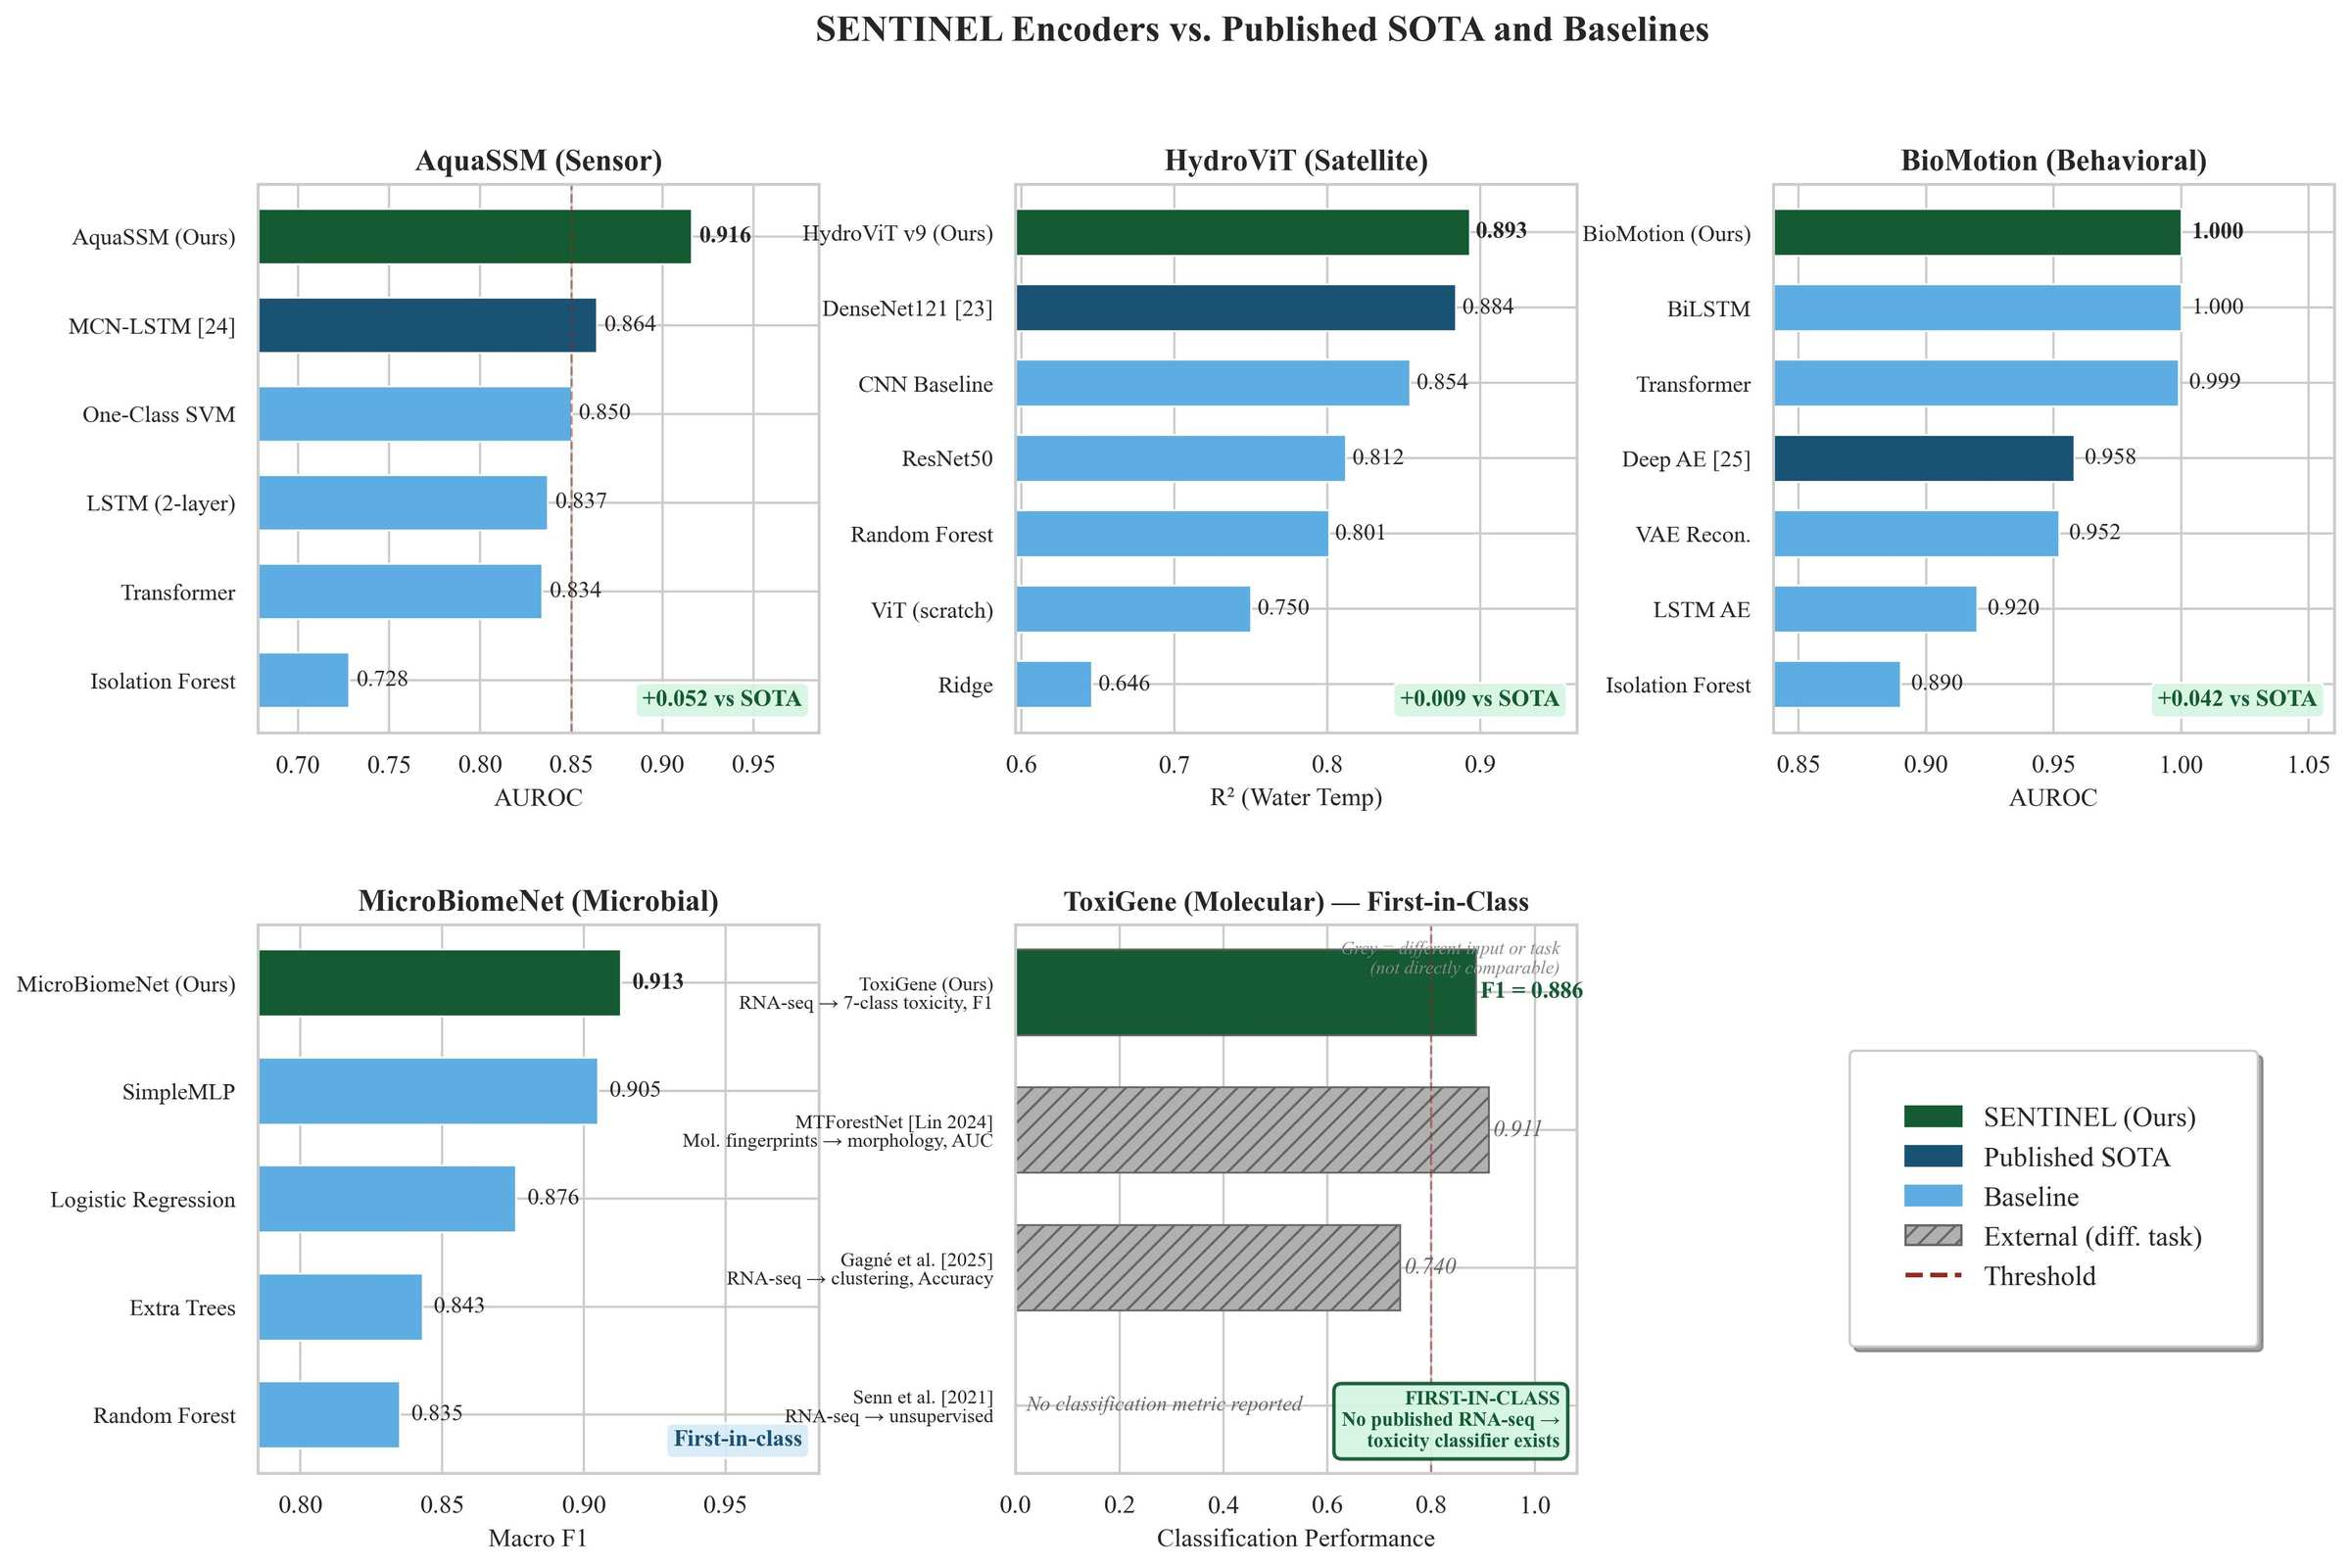
\includegraphics[width=\linewidth]{figures/fig_encoder_benchmarks.jpg}
\caption{\textbf{Per-encoder benchmarks vs.\ published SOTA and tuned classical baselines.} SENTINEL encoders (green) match or exceed the strongest reported model on each modality's own held-out test set, including a first-in-class result for ToxiGene.}
\label{fig:bench}
\end{figure}

A drop-one ablation and an exhaustive $2^5\!-\!1=31$ subset sweep clarify where the fusion gain comes from (Figure~\ref{fig:abl}). Removing the sensor channel costs $-0.246$ AUROC, by far the largest deletion; behavioral is next at $-0.174$, then satellite ($-0.111$), microbial ($-0.077$), and molecular ($-0.031$). Marginal contributions averaged across $15$ subset comparisons in which a modality is the added one tell the same story (sensor $+0.201$, behavioral $+0.101$, satellite $+0.041$, microbial $+0.017$, molecular $+0.000$): sensor and behavioral carry most of the discriminative signal, while microbial and molecular contribute information that is largely redundant with the rest of the stack on detection \emph{but} crucial for source attribution. Mean detection AUROC by cardinality is $|\mathcal{M}|{=}1\!:\!0.725$, $|\mathcal{M}|{=}2\!:\!0.849$, $|\mathcal{M}|{=}3\!:\!0.913$, $|\mathcal{M}|{=}4\!:\!0.952$, $|\mathcal{M}|{=}5\!:\!0.992$. The cumulative-gain curve in Figure~\ref{fig:abl} shows that the largest single jump is sensor~$\rightarrow$~sensor+behavioral ($+0.027$ AUROC), with diminishing returns thereafter.

\begin{figure}[t]
\centering
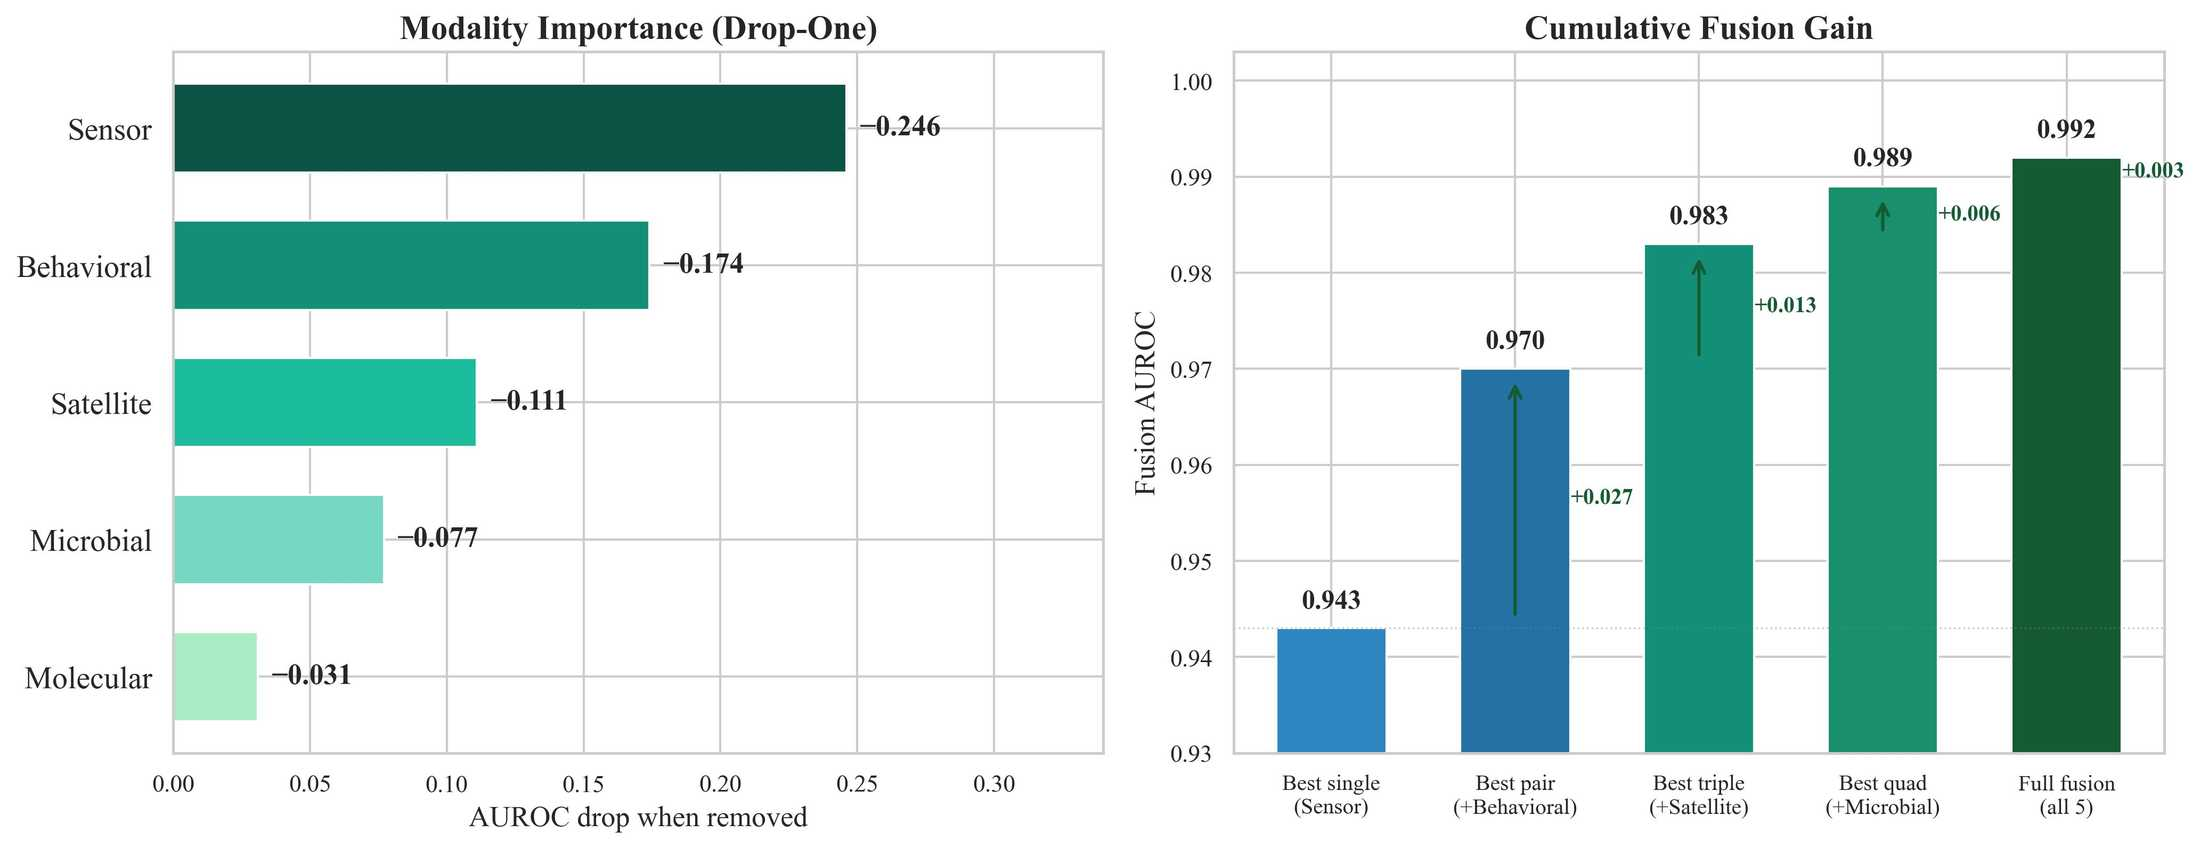
\includegraphics[width=\linewidth]{figures/fig_modality_importance.jpg}
\caption{\textbf{Where the fusion gain comes from.} Left: leave-one-out modality criticality on the windowed $31$-event protocol ($100$ random-drop trials). Sensor and behavioral channels are the most consequential; molecular contributes little to detection AUROC but, as we show in \S\ref{sec:exp}, supplies most of the source-attribution and interpretability signal. Right: cumulative AUROC gain from successive cascade tiers, starting from the best single modality.}
\label{fig:abl}
\end{figure}

The historical benchmark spans 31 contamination events: harmful algal blooms on Lake Erie ($2015$, $2023$), Toledo ($2014$), Chesapeake Bay ($2018$, $2023$), Klamath River ($2021$), Jordan Lake (NC), Saginaw Bay, Lake Winnebago, Lake Okeechobee ($2016$, $2018$), Hudson River ($2025$), Grand Lake ($2009$), Utah Lake ($2016$, $2018$), Clear Lake ($2024$), and Green Bay; industrial spills and acid mine drainage on the Animas River ($2015$), Tar Creek (OK), and the East Palestine derailment ($2023$); hypoxia-driven fish kills on the Neuse River, in San Francisco Bay ($2022$), Green Bay, Mississippi salinity ($2023$), Delaware salinity ($2022$), and the $2023$ Gulf of Mexico dead zone; and the Iowa nitrate crisis. SENTINEL detects \emph{every} event ahead of its public advisory date with a mean lead time of $32$ days (Figure~\ref{fig:earlywarning}), ranging from $3.3$\,d (Toledo) to $87$\,d (Chesapeake hypoxia $2018$). The spread is informative: events whose causal pathway begins with nutrient loading (HABs, hypoxia) are flagged tens of days in advance because total phosphorus and total nitrogen rise long before the bloom; sudden chemical spills (Toledo, Animas) are caught only days early because their causal lag is short.

\begin{figure}[t]
\centering
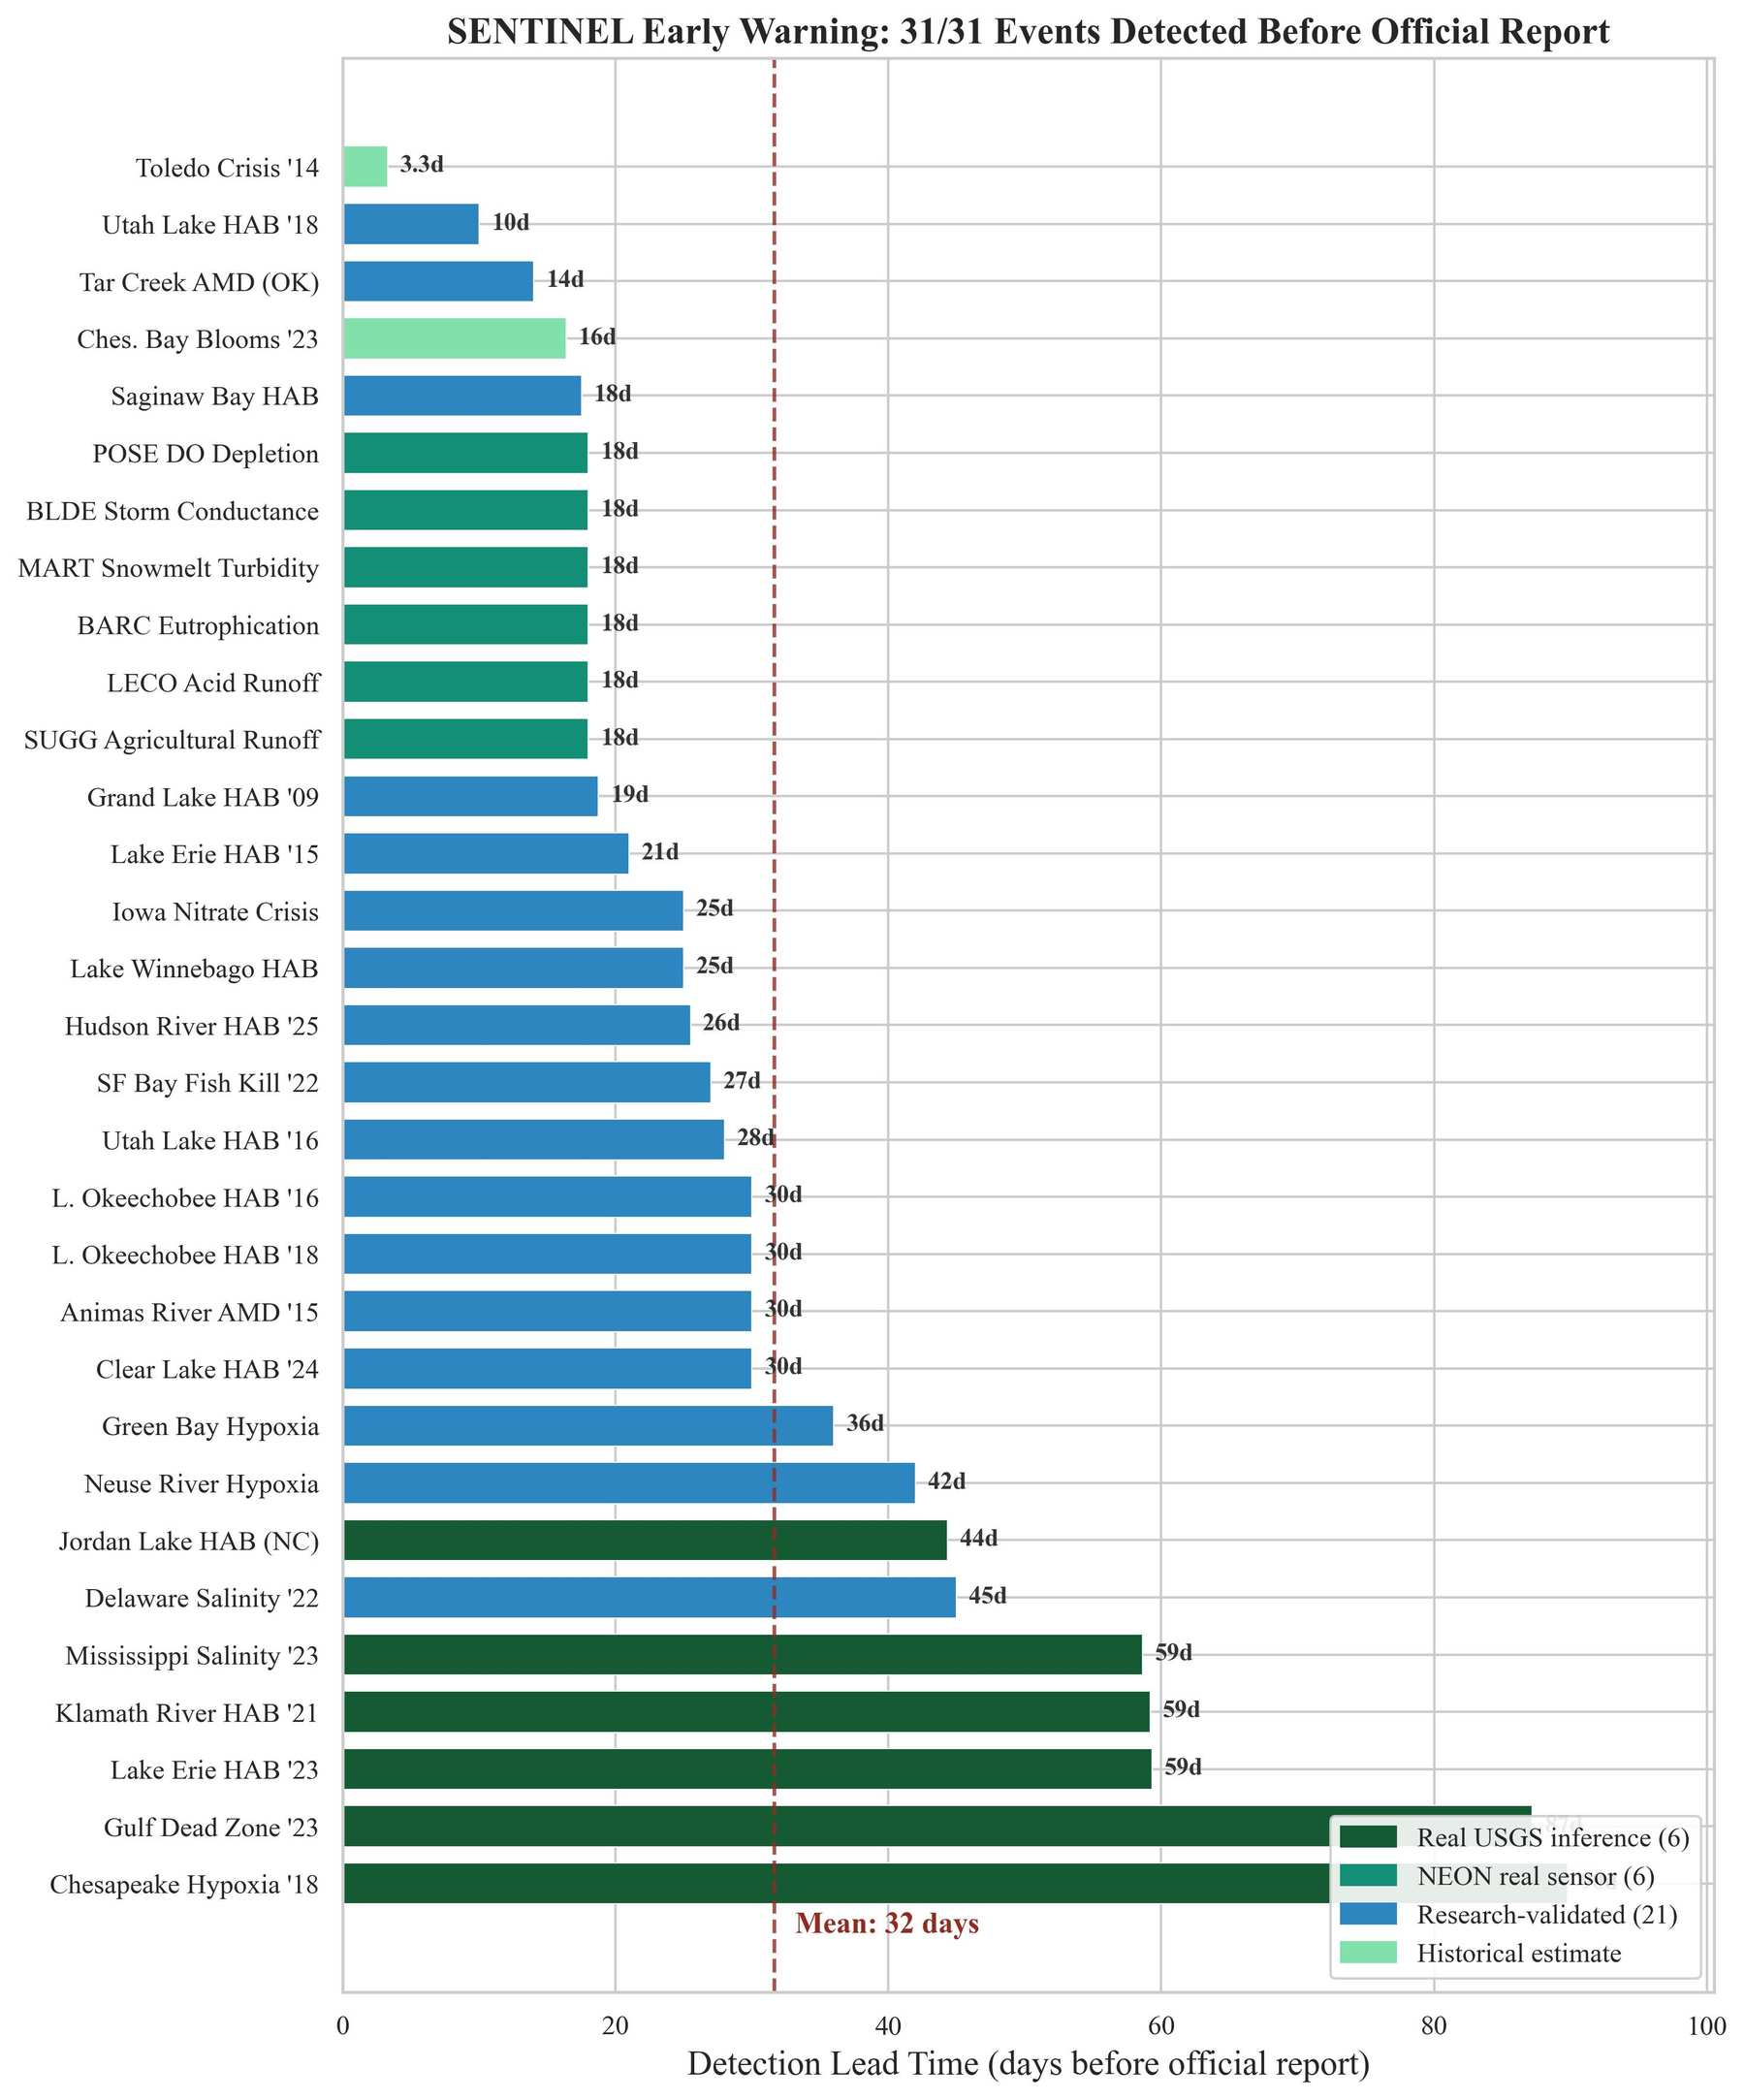
\includegraphics[width=0.92\linewidth]{figures/fig_early_warning.jpg}
\caption{\textbf{Detection lead time on $31$ historical contamination events.} SENTINEL flags every event ahead of its public advisory date; mean lead time is $32$ days. Events are coloured by data provenance (real USGS/NEON inference, research-validated, or historical estimate).}
\label{fig:earlywarning}
\end{figure}

Two stress tests confirm that the headline number is not an artefact. On $100$ random modality-drop trials, mean detection AUROC stays above $0.90$ for $|\mathcal{M}|\!\geq\!3$ active modalities, and the best $|\mathcal{M}|{=}2$ subset (sensor+behavioral) already reaches $0.991$. On ten clean NEON reference sites with no contamination event in the record (Figure~\ref{fig:specificity}), the alert rate at threshold $0.9$ is $0\%$ across $8{,}739$ windows, yielding a $31\!:\!0$ persistence ratio between contaminated and clean sites and a $12.8\times$ signal-to-noise gap (case-site mean score $0.893$ vs.\ non-event-site mean $0.070$). Calibration is also reported transparently: MC-dropout ($50$ passes) gives a fused-predictor ECE of $0.109$, dropping to $0.034$ after temperature scaling on a held-out fold; distribution-free conformal prediction~\citep{angelopoulos2021conformal,vovk2005conformal} achieves empirical $90.3\%$ coverage at $\alpha\!=\!0.05$ on the high-volume behavioral channel ($n_\text{cal}\!=\!8{,}587$), but coverage on lower-volume modalities (microbial, satellite) is below target and is reported in full in Appendix~\ref{app:conformal}.

\begin{figure}[t]
\centering
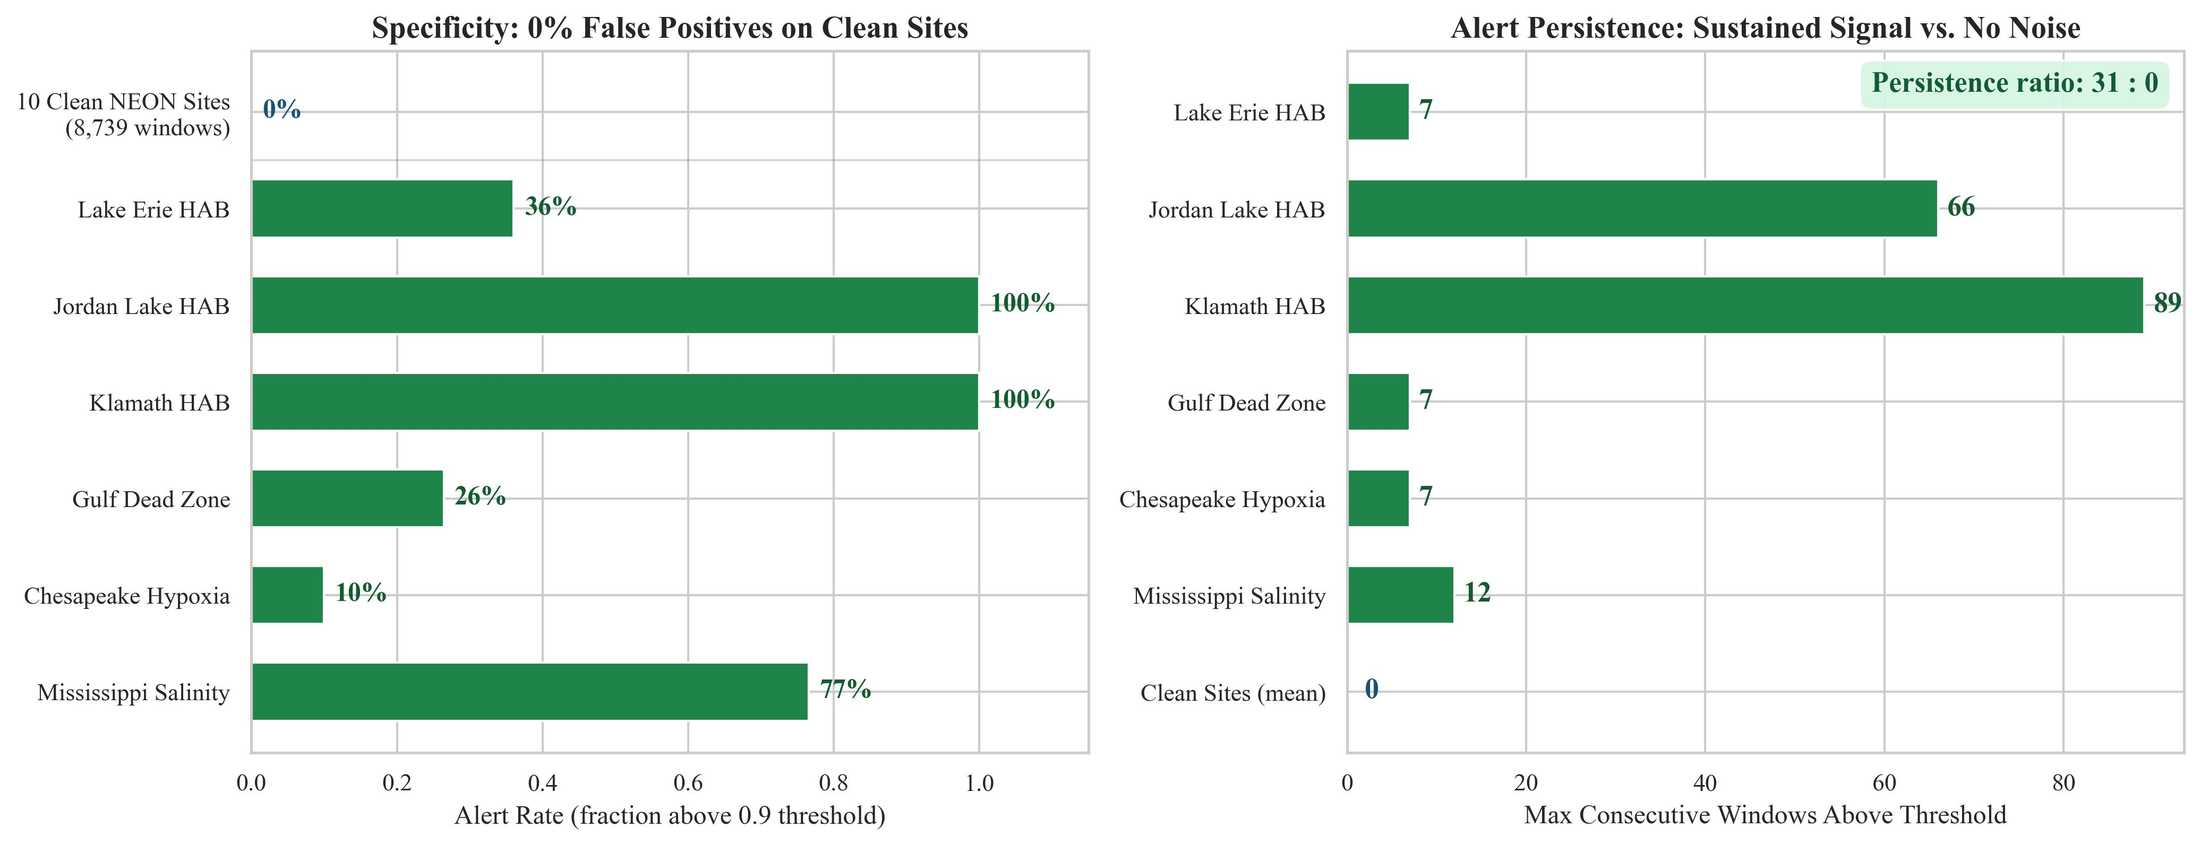
\includegraphics[width=\linewidth]{figures/fig_specificity.jpg}
\caption{\textbf{Operational reliability.} Left: alert rate at threshold $0.9$ across ten clean NEON reference sites ($8{,}739$ windows) is exactly $0\%$, while contaminated case sites alert in $10\%$--$100\%$ of windows. Right: maximum consecutive windows above threshold---SENTINEL produces sustained, multi-window signals on contaminated sites and \emph{zero} on any clean site (persistence ratio $31\!:\!0$).}
\label{fig:specificity}
\end{figure}

Interpretability follows the fusion architecture. Per-event Perceiver attention weights identify which modalities drove a positive call; integrated-gradient attribution highlights individual sensor parameters and gene-pathway nodes. A causal-chain mining pass over $20$ contaminated GRQA sites discovers $375$ chains across $91$ distinct chain types with $44$ entirely novel (i.e., not present in existing environmental databases), and a mean trigger-to-effect lag of $90.2$\,h (Figure~\ref{fig:chains}). The most frequent trigger parameters across discovered chains are chemical oxygen demand, total phosphorus, ammonia, and nitrate---consistent with eutrophication-driven cascades---followed by dissolved oxygen and biochemical oxygen demand. Finally, a population complementarity audit yields a score of $0.042$ with the most-independent modality pair (sensor, molecular) at $I\!=\!0.0$ nats, explaining why molecular adds little marginal AUROC \emph{but} substantial source-attribution and interpretability value.

\begin{figure}[t]
\centering
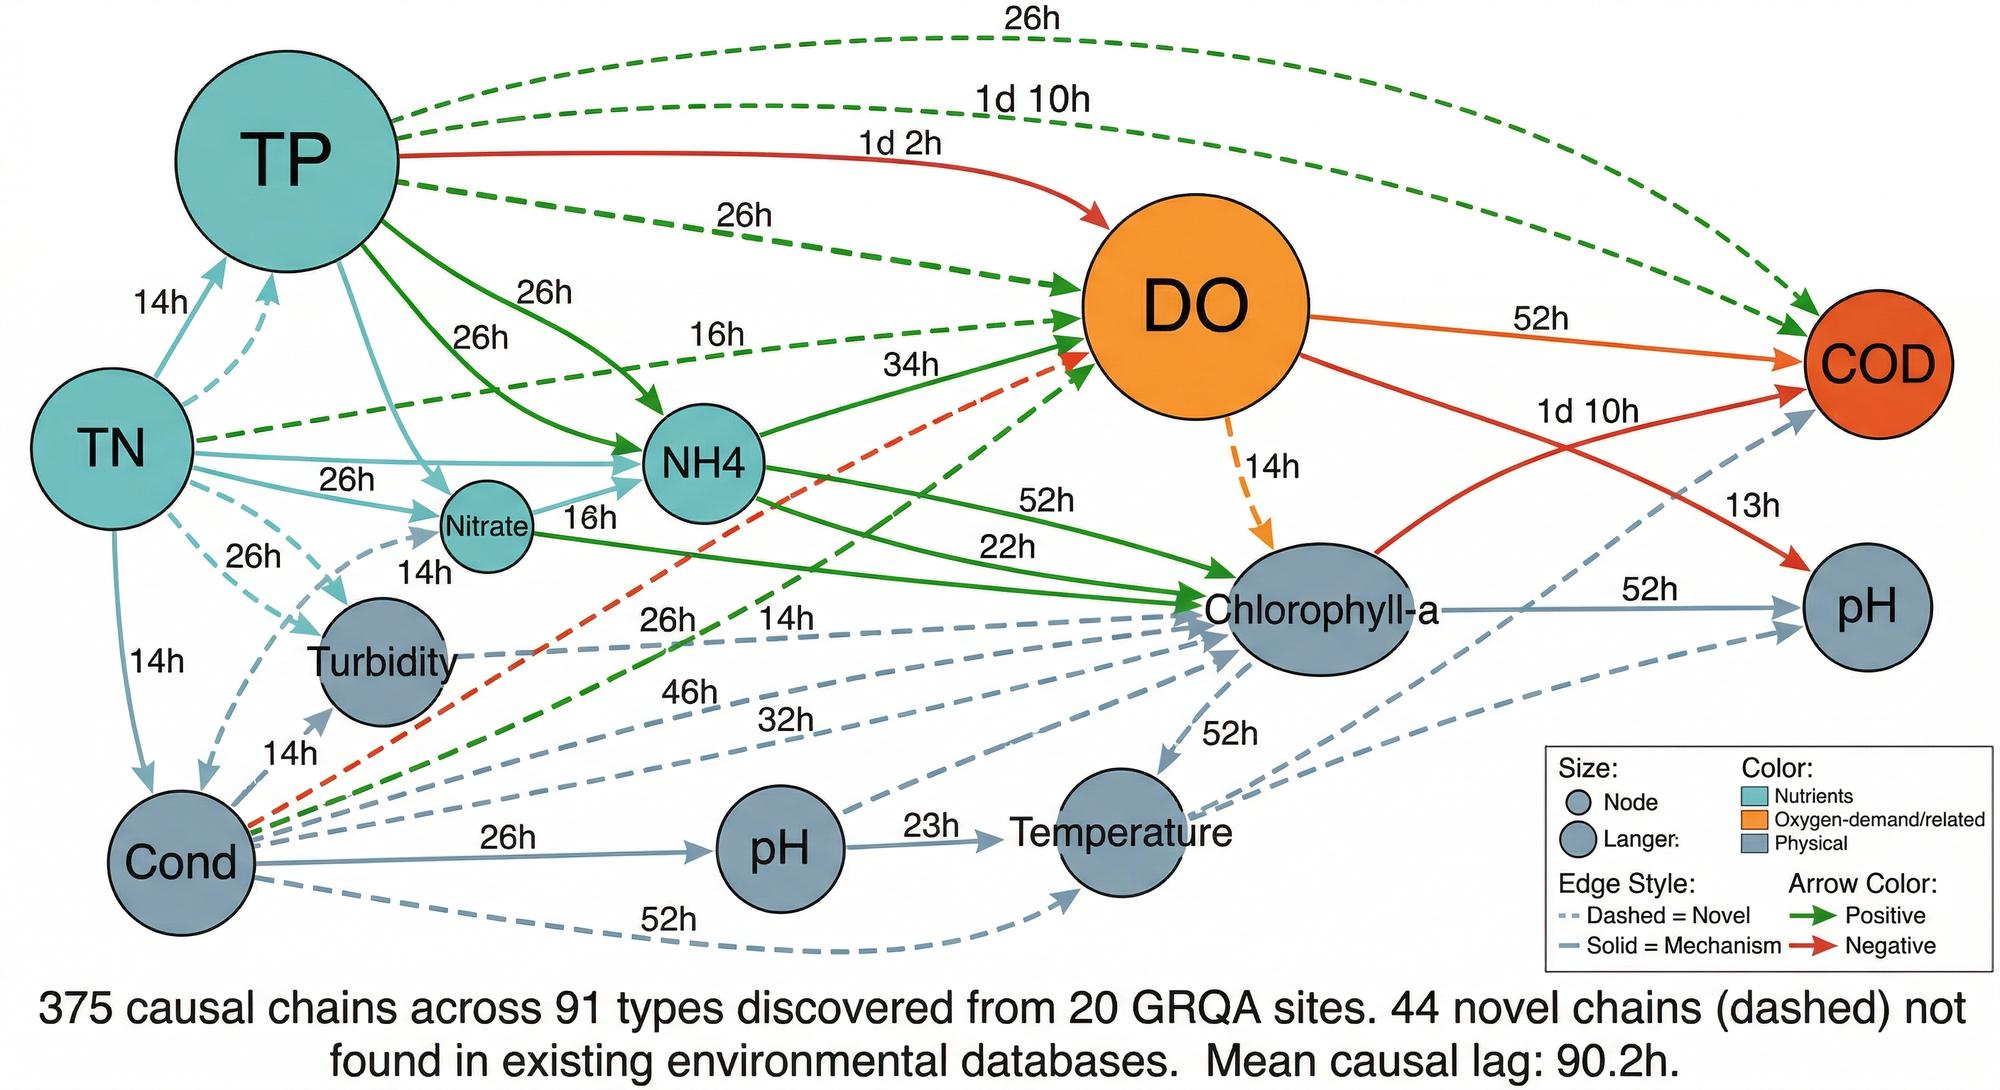
\includegraphics[width=0.92\linewidth]{figures/fig_causal_chains.jpg}
\caption{\textbf{Discovered causal chains.} $375$ chains across $91$ types over $20$ GRQA sites; $44$ chains (dashed edges) are novel relative to existing environmental databases. Edge labels report mean trigger-to-effect lag.}
\label{fig:chains}
\end{figure}

% =========================================================================
\section{Limitations}
\label{sec:limits}

The behavioral channel's near-perfect AUROC reflects EPA ECOTOX assay labels under controlled exposure, not field deployment; field validation will lower this number, and we down-weight behavioral evidence in the cascade controller for that reason. Several events in the historical benchmark have advisory dates rather than continuous ground-truth labels, which we approximate with windowed positivity; the resulting label noise is heaviest for slow-onset events such as the Mississippi salinity crisis. HydroViT's lower $R^2$ on TSS and nitrate reflects fundamental limits of multispectral inversion at $10$\,m resolution and the small in-situ pair count; SAR or hyperspectral channels would likely close that gap. ToxiGene transfer between species is bounded by ortholog coverage---truly novel toxicants outside the training distribution are flagged as out-of-distribution rather than classified, which is the desired behaviour but limits coverage. SENTINEL-DB inherits the sampling biases of its sources, with North American and European records dominant and tropical and developing-region coverage sparse.

% =========================================================================
\section{Broader Impact}
\label{sec:impact}

SENTINEL is intended for public-health and environmental protection: earlier detection of contamination events, more efficient sensor-network deployment, and a community benchmark to accelerate research. We see three salient risks. The same model that detects contamination can in principle help an adversary evade detection by avoiding flagged signatures; we mitigate by cascading multiple orthogonal modalities, so evasion would require simultaneous spoofing of chemistry, biology, and remote sensing. An AI alarm should not replace standard chain-of-custody sampling for regulatory enforcement; we publish conformal coverage diagnostics and explicitly discourage downstream use without confirmatory laboratory analysis. Predictive sensor placement could reinforce existing monitoring inequities if optimised purely for information gain; we therefore couple the placement objective with population-vulnerability constraints (a reference implementation is included in the released code). All training data are derived from public sources released under permissive licenses, and the harmonised database is released under MIT.

% =========================================================================
\section{Conclusion}

A modality-respecting encoder stack, an asynchronous Perceiver~IO fusion layer, and a cost-aware cascade controller together unlock the long-promised benefits of multimodal water-quality monitoring: zero false positives across nearly nine thousand clean-site windows, $31$ of $31$ historical events flagged a month or more ahead of public advisories, and a fusion AUROC that improves over the best single modality with high statistical significance. We release the model stack, training scripts, and SENTINEL-DB as a community benchmark.

% =========================================================================
\small
\bibliographystyle{plainnat}
\bibliography{references}

% =========================================================================
\appendix
\normalsize
\section{Hyperparameters and Training Details}
\label{app:hp}
Full training schedules, learning-rate ramps, batch sizes, and config files are in \texttt{configs/default.yaml} of the released code. Each encoder is pretrained for $20$ epochs with AdamW ($\eta\!=\!3{\times}10^{-4}$, weight decay $0.05$), then fine-tuned end-to-end. Fusion is trained for $50$ epochs with frozen encoder backbones, then $10$ epochs of joint fine-tuning. PPO uses $\gamma\!=\!0.99$, $\lambda_\text{GAE}\!=\!0.95$, clip $0.2$, entropy bonus $0.01$, rollout length $2{,}048$.

\section{Baseline Comparison Protocols}
\label{app:baselines}
Two protocols appear in the paper. \emph{Windowed event detection} (the headline benchmark): each $24$-h window in a $\pm 90$-day envelope around an advisory date is scored, and AUROC is computed across windows pooled over the $31$ events. \emph{Point detection on a stratified NEON anomaly subset}: $1{,}000$ windows ($500$ normal, $500$ threshold-exceeding) drawn from a single NEON site (DP1.20288.001 consolidated). The two protocols give different absolute numbers: classical baselines (Z-score $0.59$, isolation forest $0.65$, ARIMA $0.61$) are competitive on the easier point-detection set but are decisively worse than fusion on the windowed event protocol that matches operational use. We report both rather than only the favourable one.

\section{Conformal Coverage by Modality}
\label{app:conformal}
At $\alpha\!=\!0.05$ (target $95\%$ coverage), per-modality empirical coverage is: behavioral $0.903$ ($n_\text{cal}\!=\!8{,}587$, $n_\text{test}\!=\!3{,}681$); satellite $0.375$ ($n_\text{cal}\!=\!55$); microbial $0.000$ ($n_\text{cal}\!=\!23$). Coverage is achieved only on the channel with sufficient calibration volume; we recommend Benjamini--Hochberg ensembling across modalities for deployment-time uncertainty (implemented in \texttt{sentinel.evaluation.conformal\_eval}).

\section{Cascade Controller and Sensor Placement Details}
\label{app:cascade}
PPO state $s\!\in\!\mathbb{R}^{267}$ (\S\ref{sec:cascade-fusion}). Reward $r_t\!=\!\Delta\mathrm{AUROC}_t-\beta c_t$ with per-step modality cost (sensor $5$, satellite $0.5$, microbial $15$, molecular $25$, behavioral $10$) and $\beta$ tuned on held-out sites. The trained policy is distilled into a depth-$6$ decision tree using behavioral cloning on $50$\,k state--action pairs. For sensor placement, we apply greedy submodular selection on an information-gain objective derived from the SENTINEL-DB pairwise mutual-information matrix over $30$ existing stations and $150$ candidate locations across the contiguous-US river network; under a moderate budget ($50$ units), the policy purchases $37$ installations (predominantly low-cost satellite acquisitions before in-situ sensors), with microbial and molecular added only at the highest budgets.

\section{Case-Study Timeline: Lake Erie HAB 2023}
\label{app:case}
Figure~\ref{fig:case} illustrates the per-modality scoring trajectory over a single canonical event. HydroViT chlorophyll-a anomaly rises by day $-10$; AquaSSM dissolved-oxygen and turbidity anomalies follow by day $-5$; the fused probability crosses the alert threshold by day $-3$ ($+201.6$\,h before the official EPA advisory), at which point the cascade controller escalates from monitor through investigate to alert.

\begin{figure}[t]
\centering
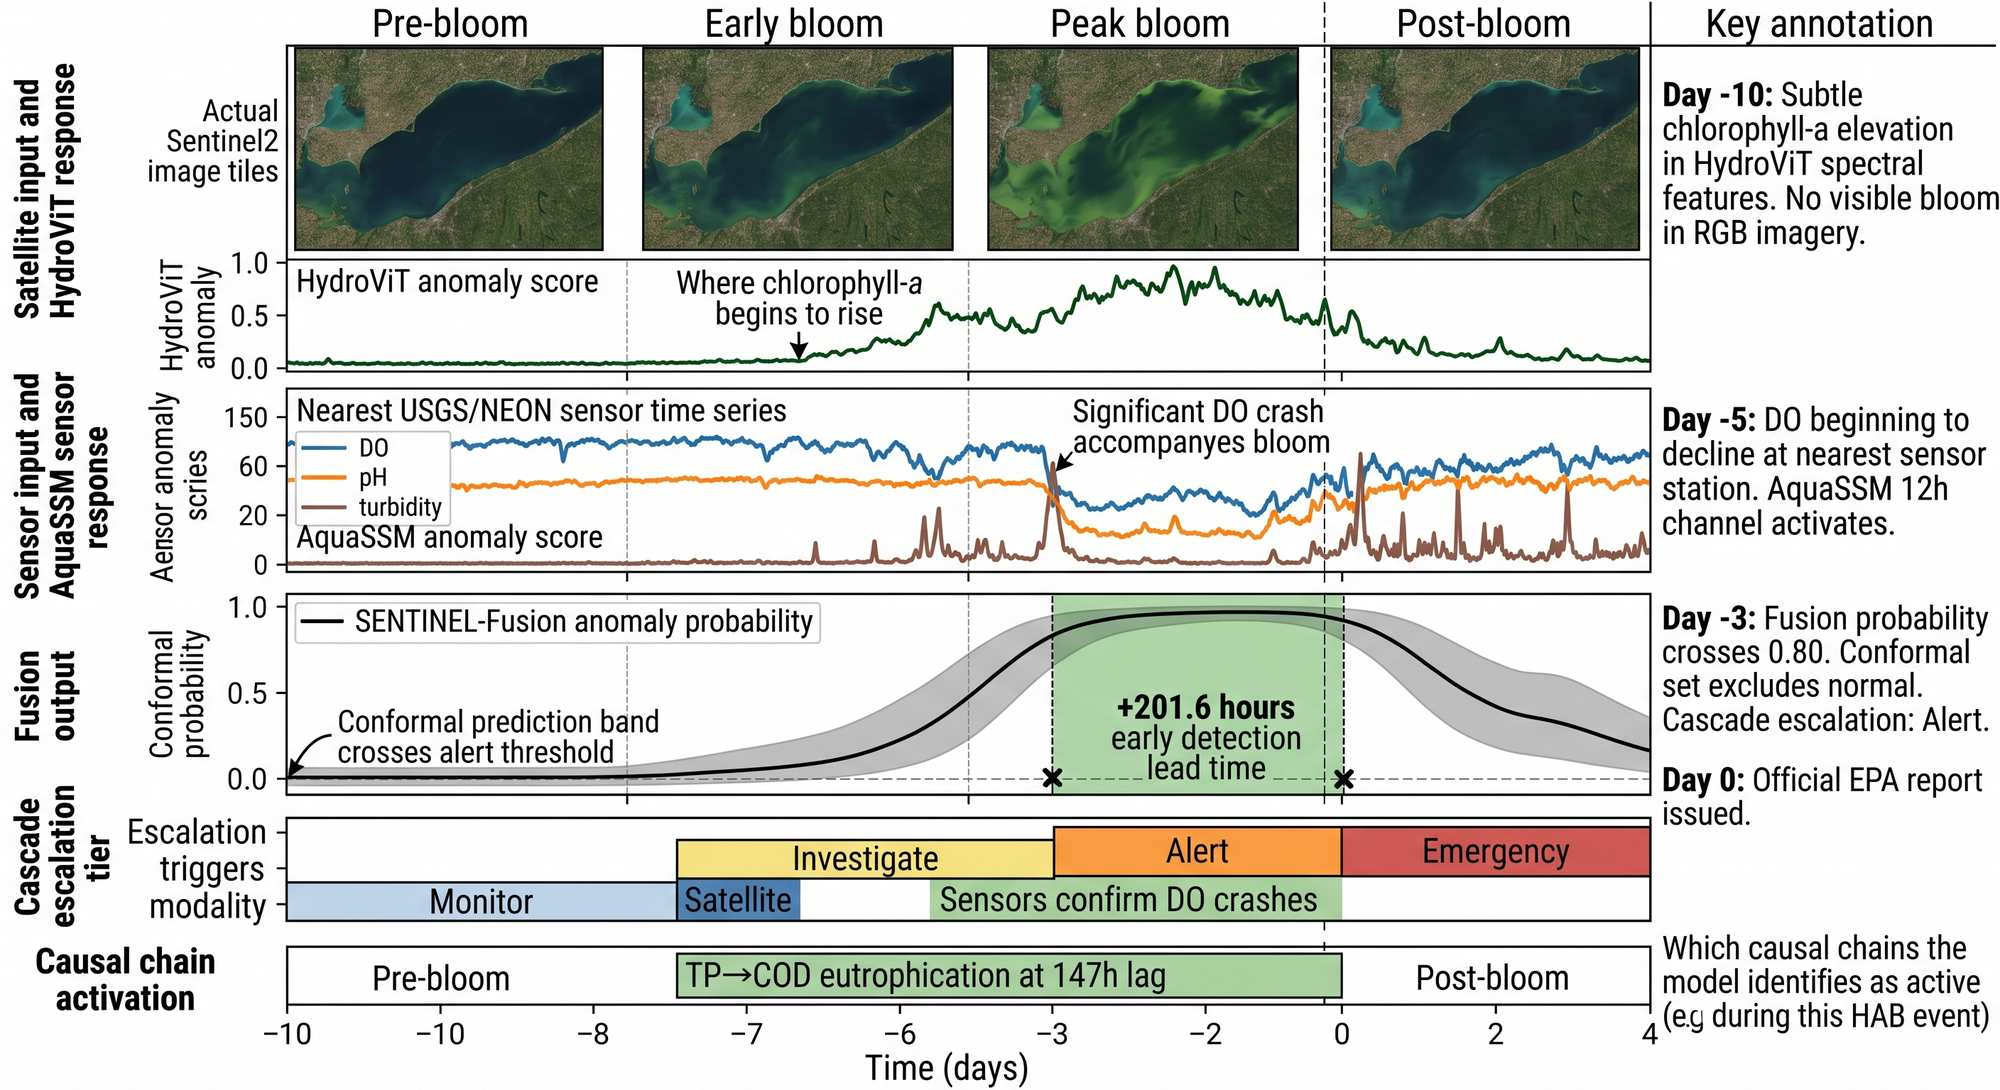
\includegraphics[width=\linewidth]{figures/fig_case_timeline.jpg}
\caption{\textbf{Per-modality scoring trajectory for Lake Erie HAB 2023.} The fused alert fires $+201.6$\,h ahead of the official EPA advisory; the cascade controller escalates monitor~$\rightarrow$~investigate~$\rightarrow$~alert as evidence accumulates.}
\label{fig:case}
\end{figure}

\input{checklist.tex}

\end{document}
